\documentclass{beamer}
\usetheme{Madrid}
\usepackage{array}
\title[MAT 206 M1]{GRAPH THEORY}
\subtitle{Module 1}
\author{Rijin IK}
\institute[VJEC]{Assistant Professor\\Department of Computer Science and Engineering\\Vimal Jyothi Engineering College\\Chemperi}
\begin{document}
	\begin{frame}
		\titlepage
	\end{frame}
   \begin{frame}{Outline}
   \tableofcontents
   \end{frame}
\section{Introduction to Graphs}
\begin{frame}{Introduction to Graphs}
\begin{block}{Graphs}
	\begin{itemize}
		\item 	A graph G = (V, E) consists of a set of objects V=\{v1, v2, v3, … \} called vertices (also 
		called points or nodes)
		\item and other set E = \{e1, e2, e3, .......\} whose elements are called edges 
		(also called lines or arcs).
	\end{itemize}
\end{block}
\begin{itemize}
	\item The set V(G) is called the vertex set of G and E(G) is the edge set of G.
	\item A graph is denoted as G=(V,E)
\end{itemize}
\begin{figure}
	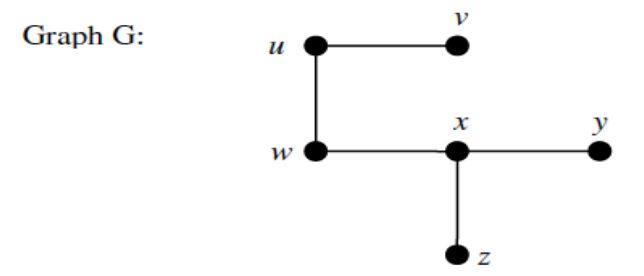
\includegraphics[scale=.45]{img/m1}
\end{figure}
Graph G with 6 vertices and 5 edges
\end{frame}
\begin{frame}{Introduction to Graphs}
	\begin{itemize}
		\item A graph with p-vertices and q-edges is called a (p, q) graph.
	\end{itemize}
	\textbf{Trivial Graph}
	\begin{itemize}
		\item A graph is said to be trivial if a finite graph contains only one vertex and no edge.
		\item The (1, 0) graph is called trivial graph. 
		\begin{figure}
			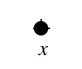
\includegraphics[scale=.5]{img/m3}
		\end{figure}
	\end{itemize}
	\textbf{Self-loop.}
	\begin{itemize}
		\item An edge having the same vertex as its end vertices is called a self-loop.
		\begin{figure}
			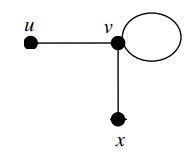
\includegraphics[scale=.5]{img/m2}
		\end{figure}
	\end{itemize}
\end{frame}
\begin{frame}{Introduction to Graphs}
	\textbf{Parallel edges.}
	\begin{itemize}
		\item More than one edge associated a given pair of vertices called parallel edges.
		\begin{figure}
			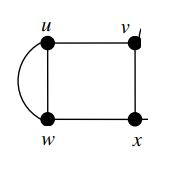
\includegraphics[scale=.5]{img/m4}
		\end{figure}
	\end{itemize}
	\textbf{Simple graph.}
\begin{itemize}
	\item A graph that has neither self-loops nor parallel edges is called simple graph.
	\begin{figure}
		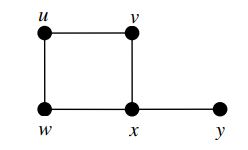
\includegraphics[scale=.5]{img/m5}
	\end{figure}
\end{itemize}
\end{frame}
\begin{frame}{Introduction to Graphs}
	\textbf{ Multigraph.}
	\begin{itemize}
		\item Any graph which contain some parallel edges but doesn’t contain any self-loop is called multi graph. 
		\begin{figure}
			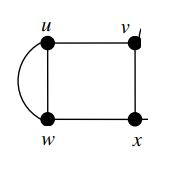
\includegraphics[scale=.5]{img/m4}
		\end{figure}
	\end{itemize}
	\textbf{Pseudo Graph.}
	\begin{itemize}
		\item A graph that may contain self loop as well as parallel edge is called a pseudo graph.
		\begin{figure}
			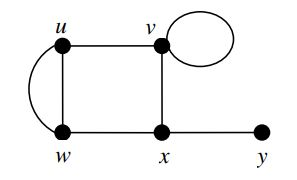
\includegraphics[scale=.5]{img/m6}
		\end{figure}
	\end{itemize}
\end{frame}
\begin{frame}{Introduction to Graphs}
	\textbf{Un-directed graph.}
	\begin{itemize}
		\item If an edge consist of unordered pair of elements of V, then the graph is called Un-directed graph.
		\item In other words, if each edge of the graph G has no direction then the graph is called un-directed
		graph.
		\begin{figure}
			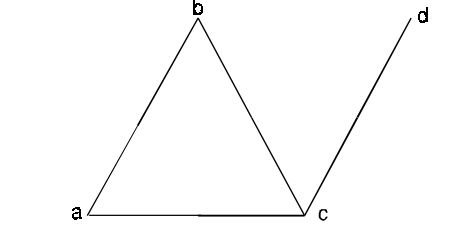
\includegraphics[scale=.3]{img/m7}
		\end{figure}
	\end{itemize}
	\textbf{Directed graph.}
	\begin{itemize}
		\item If an edge contain ordered pair of elements of V, then the graph is called Directed graph.
		\item In other words, if each edge of the graph G has a direction then the graph is called directed
		graph.
		\begin{figure}
			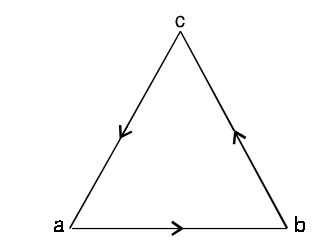
\includegraphics[scale=.3]{img/m8}
		\end{figure}
	\end{itemize}
\end{frame}
\section{Application of graphs}
\begin{frame}{Application of graphs}
\textbf{Konigsberg bridge problem}
\begin{itemize}
	\item Two islands C and D were connected to
	each other and to the banks A and B with seven bridges as shown in
	figure. 
	\item The problem was to start at any land areas A, B, C or D , walk
	over each of the seven bridges exactly once, and return to the starting
	point
	\begin{figure}
		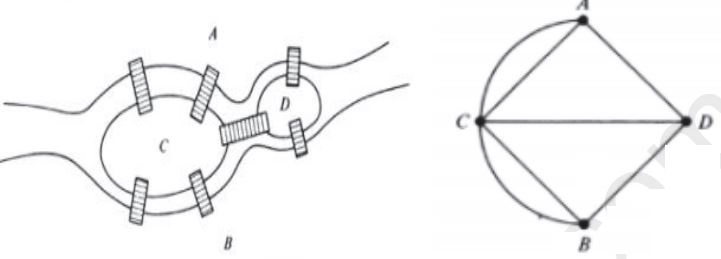
\includegraphics[scale=.4]{img/m10}
	\end{figure}
\item Euler represented this problem by means of a graph. Vertices
represent the land areas and the edges represents the bridges.
\item Euler proved that a solution for this problem does not exists
\end{itemize}
\end{frame}
\begin{frame}{Application of graphs}
	\textbf{Utilities problem}
	\begin{itemize}
		\item There are three houses H1, H2 and H3, each to be connected to each of the three
		utilities water (W), gas (G) and electricity (E) by means of conduits. 
		\item Is it possible to make such connection without any crossover of the conduits?
		\begin{figure}
			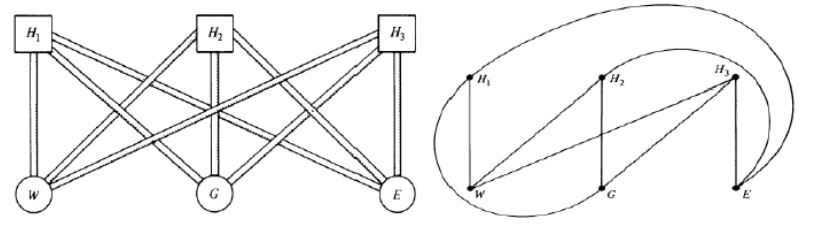
\includegraphics[scale=.4]{img/m11}
		\end{figure}
		\item A solution for this problem does not exists.
		\item The graph cannot be drawn in a plane without any edge cross-over
	\end{itemize}
\end{frame}
\begin{frame}{Application of graphs}
	\textbf{Seating problem}
	\begin{itemize}
		\item Nine members of a new club meet each day for lunch at a round table. They decide
		to sit such that every member has different neighbors at each lunch.
		\item  How many days can this arrangement last?
		\begin{itemize}
			\item This situation can be represented by a graph with nine vertices such that each vertex
			represents a member, and an edge joining two vertices represents the relationship of sitting
			next to each other
		\end{itemize}
		\begin{figure}
			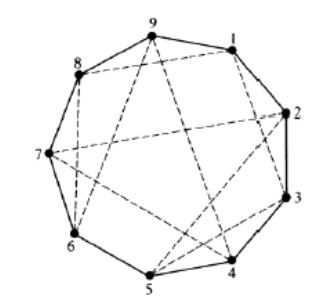
\includegraphics[scale=.3]{img/m12}
		\end{figure}
		\item  Figure shows two possible seating arrangements
		\begin{itemize}
			\item 1 2 3 4 5 6 7 8 9 1 (solid lines)
			\item 1 3 5 2 7 4 9 6 8 1 (dashed lines).
			\begin{itemize}
				\item  It can be shown by graph-theoretic
				considerations that there are more arrangements possible.
			\end{itemize}
		\end{itemize}
	\end{itemize}
\end{frame}

\begin{frame}{Application of graphs}
	\textbf{Seating problem:A solution exists or not?}
	\begin{itemize}
		\item Yes
		\item 4 seating arrangements are possible.
	\end{itemize}
for n people ,the number of possible arrangement is 
\begin{itemize}
	\item $\frac{n-1}{2}$ , if n is odd
	\item $\frac{n-2}{2}$ ,if n is even
	
\end{itemize}
		
\end{frame}


\begin{frame}{Application of graphs}
	\textbf{Electrical Network Problem.}
	\begin{itemize}
		\item Topology of a electrical network is
		studied by means of graphs. 
		\item Vertices represented the electrical
		network junctions and the edges represented the branches.
		\begin{figure}
			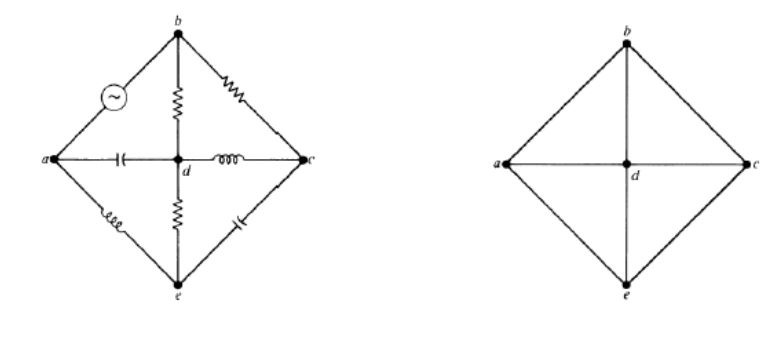
\includegraphics[scale=.5]{img/m13}
		\end{figure}
	\end{itemize}
\end{frame}
\begin{frame}{Finite and Infinite Graph}
	\textbf{Finite and Infinite Graph}
\begin{itemize}
	\item A graph with finite number of vertices and finite number of edges is 
	called a finite graph, otherwise it is an infinite graph
\end{itemize}
	\begin{figure}
	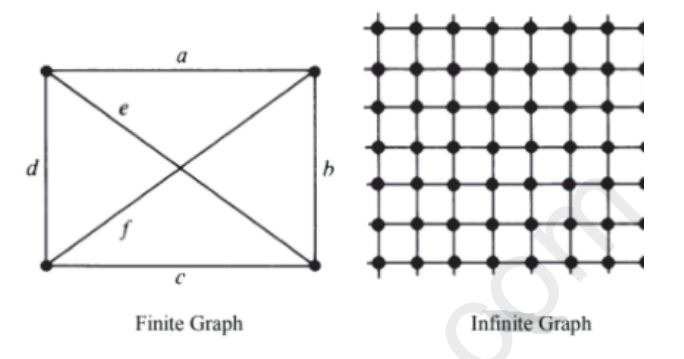
\includegraphics[scale=.5]{img/m14}
\end{figure}
\end{frame}
\begin{frame}{Bipartite graphs}
	\begin{block}{Bipartite graphs}
		A graph G is bipartite if the node set V can be partioned into two sets $V_1$ and $V_2$ in such a way that no nodes from the same set are adjacent
	\end{block}
\begin{columns}
	\begin{column}{.5\textwidth}
			\begin{figure}
			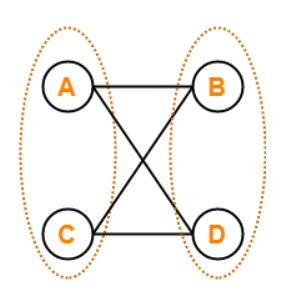
\includegraphics[scale=.5]{img/m15}
		\end{figure}
	\end{column}
		\begin{column}{.5\textwidth}
		\begin{figure}
			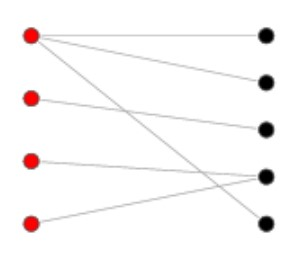
\includegraphics[scale=.5]{img/m39}
		\end{figure}
	\end{column}
	
\end{columns}

\begin{itemize}
	\item The vertices of the graph can be decomposed into two sets.
	\item The two sets are X = \{A, C\} and Y = \{B, D\}.
	\item The vertices of set X join only with the vertices of set Y and vice-versa.
	\item The vertices within the same set do not join.
\end{itemize}
\end{frame}
\begin{frame}{Bipartite graphs}
	\textbf{Complete Bipartite Graph}
	\begin{itemize}
		\item A bipartite graph where every vertex of set X is joined to every vertex of set Y
		is called as complete bipartite graph.
	\end{itemize}
	\begin{figure}
		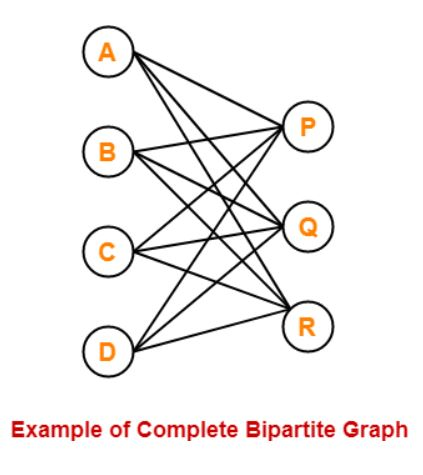
\includegraphics[scale=.5]{img/m16}
	\end{figure}
\end{frame}
\section{Incidence and Degree}
\begin{frame}{Incidence and Degree}
	\textbf{Incidence}
	\begin{itemize}
		\item When a vertex $v_i$ is an end vertex of some edge $e_j$, $v_i$ and $e_j$ are said to incident with each other.(edge touches that vertices) 
		\item Two non parallel edges said to be \textbf{\textit{adjacent}} if 
		they are incident on a common vertex.
	\end{itemize}
	\begin{figure}
	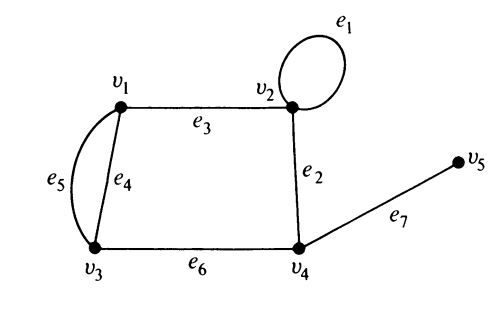
\includegraphics[scale=.5]{img/m17}
\end{figure}
\begin{itemize}
	\item $e_3,e_4,e_5 \ incident\  on\  the\  vertex\  V_1$
		\item $e_3,e_1,e_2 \ incident\  on\  the\  vertex\  V_2$
	\item $e_4,e_5,e_6 \ incident\  on\  the\  vertex\  V_3$
	\item $e_7 \ incident\  on\  the\  vertex\  V_5$
\end{itemize}
\end{frame}
\begin{frame}{Incidence and Degree}
	\textbf{Degree or valency of a vertex}
	\begin{itemize}
		\item The number of edges incident on a vertex $v_i$, with self loop counted 
		twice, is called the degree  d($v_i$) of vertex $v_i$.
		\item  For example:
		\begin{itemize}
			\item d($v_1$)= d($v_3$)= d($v_4$)=3
			\item d($v_2$)=4
			\item d($v_5$)=1
		\end{itemize}
	\end{itemize}
	\begin{figure}
		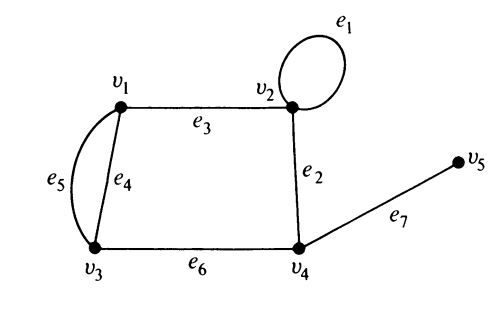
\includegraphics[scale=.6]{img/m17}
	\end{figure}
A graph in which all vertices are of equal 
degree is called \textbf{regular graph} 
\end{frame}

\begin{frame}{Incidence and Degree}
	\textbf{Regular graph}
	\begin{itemize}
		\item 	A graph in which all vertices are of equal 
		degree is called \textbf{regular graph} 
		Regular graph with 3 vertices; d(V1)=d(V2)=d(V3)=2
		\begin{itemize}
			\item A regular graph with degree two is called 2-Regular graph (A regular graph with degree k is called k-Regular graph)
		\end{itemize}
	
	\end{itemize}
	\begin{figure}
	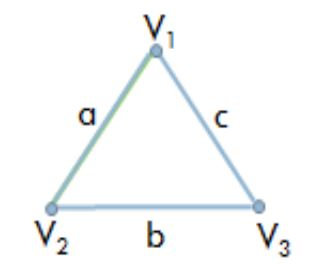
\includegraphics[scale=.23]{img/m29}
\end{figure}
\textbf{Complete graph}
\begin{itemize}
	\item A graph in which there exists an edge between every pair of vertex is 
	called a complete graph.
\end{itemize}
\begin{figure}
	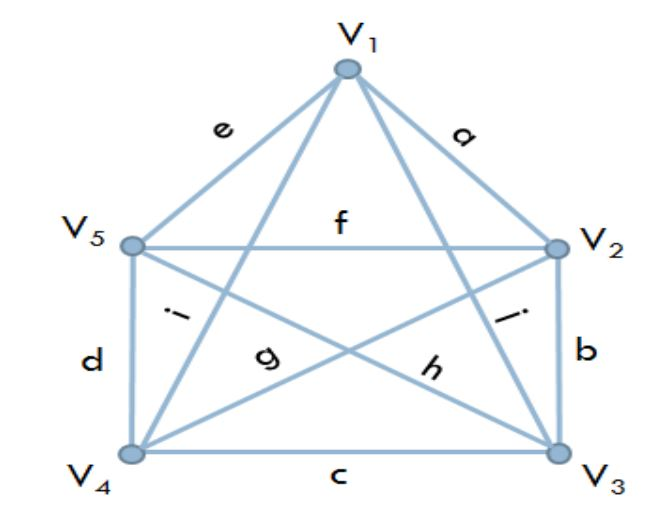
\includegraphics[scale=.23]{img/m30}
\end{figure}
\end{frame}


\begin{frame}{Incidence and Degree}
\begin{block}{Handshaking Lemma}
Sum of degrees of all vertices in G is twice the number of edges in G
	$$\sum_{i=1}^{n}d(v_i)=2e$$
\end{block}
	\begin{figure}
	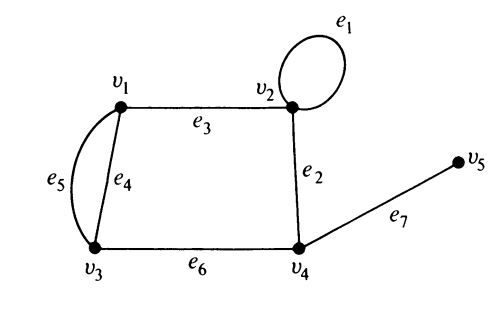
\includegraphics[scale=.4]{img/m17}
\end{figure}
\begin{equation*}
	\begin{array}{c c c}
		sum \ of\  degrees\  of\  vertices &=&d(v1)+d(v2)+d(v3)+ d(v4)+d(v5)\\
		&=& 3+4+3+3+1\\
		&=&14\\ &=&twice\  the\  number\  of\  edges
	\end{array}
\end{equation*}
\end{frame}

\begin{frame}{Incidence and Degree}
	\begin{block}{Theorem1.1:}
	The number of vertices of odd degree in a graph is always even
	\end{block}
	\begin{figure}
		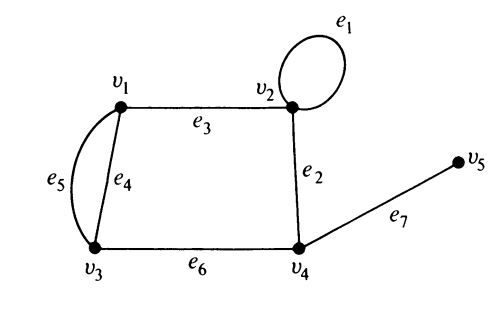
\includegraphics[scale=.4]{img/m17}
	\end{figure}
	\begin{equation*}
		\begin{array}{c c c}
			the\ number \ of\  vertices \ of\  odd \ degree &=&d(v1),d(v3),d(v4),d(v5)\\
			&=& 3,3,3,1\\
			&=& 4(even)\\
		\end{array}
	\end{equation*}
\end{frame}
\begin{frame}{Incidence and Degree}
	\textbf{The number of vertices of odd degree in a graph is always even}	\\
(Proof)Sum of the degrees of all vertices in G
	\begin{eqnarray}
	\sum_{i=1}^{n} d(v_i) &=& 2e
		\end{eqnarray}
	If we consider the vertices with odd and even degree separately.
	\begin{small}
		\begin{eqnarray}
		\sum_{i=1}^{n} d(v_i) &=& \sum_{even} d(v_j)+\sum_{odd} d(v_k)\\
		\sum_{even} d(v_j)+\sum_{odd} d(v_k)&=& 2e\\
		even\ +\sum_{odd} d(v_k)&=& even\\
		\sum_{odd} d(v_k)&=& even-even\\
		\sum_{odd} d(v_k)&=& even
	\end{eqnarray}
	\end{small}
\end{frame}
\begin{frame}{Incidence and Degree}
	\textbf{Find if a degree sequence can form a simple graph}
	\begin{itemize}
		\item[i] Sort the degrees in descending order
		\item[ii] Delete the first element(say V). Subtract 1 from the next V elements.
		\item[iii] Repeat 1 and 2 until one of the stopping conditions is met.
	\end{itemize}
	\textbf{Stopping conditions:}
	\begin{itemize}
		\item[a] All the elements remaining are equal to 0 (Simple graph exists).
		\item[b] Negative number encounter after subtraction (No simple graph exists).
		\item[c] Not enough elements remaining for the subtraction step (No simple graph exists).
	\end{itemize}
\textbf{Q1:}Can there be a graph with degree sequence 3 2 2 1
\end{frame}
\begin{frame}{Incidence and Degree}
	\textbf{Constructing a graph from a degree sequence}
	\begin{itemize}
		\item[i] Sort the degrees in descending order
		\item[ii] Connect the highest degree d to the next d vertices
		\item[iii] Take away(remove) the first degree (value of d) and reduce the 
		following d degrees by one
		\item[iv] Repeat the steps until all degrees are zero
	\end{itemize}
	
\end{frame}
\begin{frame}{Incidence and Degree}
	\begin{itemize}
		\item[Q1:] How many edges are there in a graph with 10 vertices and each 
		of degree 6 ? 
			\item[Q2:] Draw graphs representing problems of
			\begin{itemize}
				\item[a] two houses and three utilities;
				\item[b] four houses and four utilities, say, water, gas, electricity, and
				telephon
			\end{itemize} 
		\item[Q3] A graph has 5 vertices with degree as:
		a. 2,3,1,1,2 check the given degree sequence form a graph
		\item[Q4] Can there be a graph with degree sequence (5, 5, 4, 3, 2, 1)
		\item[Q5] Can there be a graph with degree sequence (1, 1, 1)? Explain.
		\item[Q6] Could there exist a graph with the following degrees of vertices: (a) 4, 3, 3, 1 (b) 4, 3,3,2,2 (c) 5,4,4,2,2,1? (If yes, can we provide an example and If no, can we explain why?
		\item[Q7] There are 25 telephones in CSE Dept. Is it possible to connect them with wires so that each telephone is connected with exactly 7 others. 
	\end{itemize}
\end{frame}
\begin{frame}{Incidence and Degree}
	\begin{itemize}
			\item[HW1:] Convince yourself that the maximum degree of any vertex in a simple
		graph with n vertices is n – 1.
		\item[HW2:]  Show that the maximum number of edges in a simple graph with n
		vertices is $\frac{n(n – l)}{2}$.
		\item[HW3:] Draw the graph of the Wheatstone bridge circuit.
		\item[HW4:] Draw graphs of the following chemical compounds:$ (a) CH_4, (b) C_2H_6,(c) C_6H_6,(d)N_2O_3.$(Hint: Represent atoms by vertices and chemical bonds between them by edges.)
		\item[HW5:] Draw a graph with 64 vertices representing the squares of a chessboard.
		Join these vertices appropriately by edges, each representing a move of
		the knight. You will see that in this graph every vertex is of degree two,
		three, four, six, or eight. How many vertices are of each type?
	
	\end{itemize}
\end{frame}
\begin{frame}{Incidence and Degree}
\textbf{Q1:}Show that the maximum number of edges in a simple graph with n
vertices is $\frac{n(n – l)}{2}$.
\begin{itemize}
	\item We have that is a simple graph, no parallel or loop exist. Therefore the degree of each vertex will be one less than the total number of vertices (at most). ie, degree=n-1.
	\item We know that the sum of the degree in a simple graph always even ie, $$\sum_{i=1}^{n} d(v_i) = 2e$$
	here d(v)=n-1 : we have n vertices the total degree is n(n-1) $$n(n-1)=2E$$
	$$E=\frac{n(n-1)}{2}$$
\end{itemize}
\end{frame}
\section{Isolated vertex, Pendant vertex and NULL Graph}
\begin{frame}{Isolated vertex \& Pendant vertex}
	\textbf{Isolated vertex}
	\begin{itemize}
		\item A vertex having no incident edge is called isolated vertex.
		\item Isolated 
		vertices are vertices with zero degree.
	\end{itemize}
\textbf{Pendant vertex}
\begin{itemize}
	\item A vertex of degree one is called a pendant vertex or an end 
	vertex.

\end{itemize}
\begin{figure}
	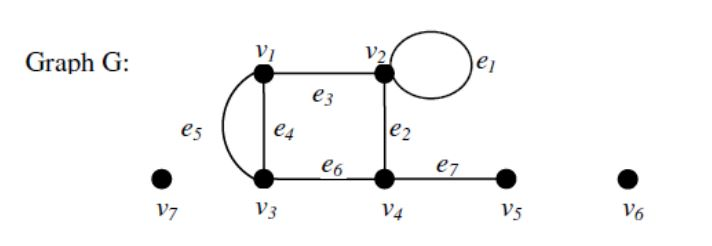
\includegraphics[scale=.4]{img/m18}
\end{figure}
\begin{itemize}
	\item The vertices $v_6$ and $v_7$ are isolated vertices.
	\item The vertex $v_5$ is a pendant vertex.
\end{itemize}
\end{frame}
\begin{frame}{Null graph}
	\textbf{Null graph}
	\begin{itemize}
		\item A graph without any edges is called null graph
		\item Every vertex in null graph is an isolated vertex
	\end{itemize}
\begin{figure}
	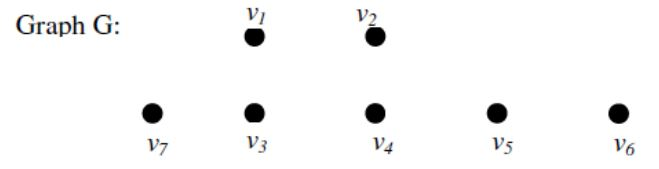
\includegraphics[scale=.4]{img/m19}
\end{figure}
\end{frame}
\section{Isomorphism}
\begin{frame}{Isomorphism}
	\begin{block}{Isomorphism}
		Two graphs G and G' are said to be isomorphic to each other if there is a one-to one
		correspondence (bijection) between their vertices and between their edges such that the incidence 
		relationship is preserved.
	\end{block}
\textbf{The two isomorphic graph must have}
\begin{itemize}
	\item same number of vertices
	\item same number of edges
	\item equal number of vertices with a given degree
\end{itemize}
\end{frame}
\begin{frame}{Isomorphism}
	\textbf{QN: Check whether the following pair of graphs are 
		isomorphic or not}
	\begin{figure}
		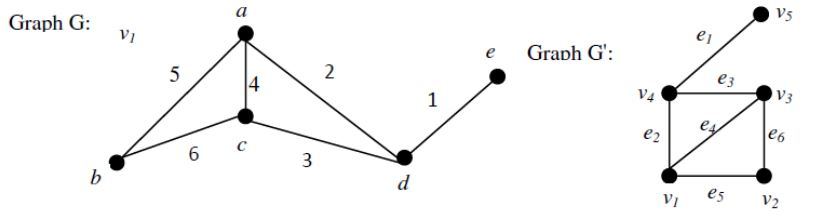
\includegraphics[scale=.4]{img/m20}
	\end{figure}
\begin{small}
	\begin{table}
		\begin{tabular}{| p{4cm} | p{3cm} | p{3cm} |}
			\hline
			& G1 & G2\\ \hline
			Vertices & \{a,b,c,d,e\} & \{v1,v2,v3,v4,v5\}\\ \hline 
			Total no. of vertices & 5 & 5\\ \hline 
			Vertices with degree 
			(arranged in
			decending order) &
			a, c, d, b, e & v1, v3, v4, v2, v5\\\hline
			Total number of edges= 
			sum of
			degrees of all vertices/2 & $(3+3+3+2+1)/2=6$ & $(3+3+3+2+1)/2=6$\\
			\hline
		\end{tabular}
	\end{table}
Since G1 and G2 have same number of vertices and same number of edges, G1 and G2 are
isomorphic Graphs
\end{small}
\end{frame}
\begin{frame}{{Isomorphism}}
	
	\begin{figure}
		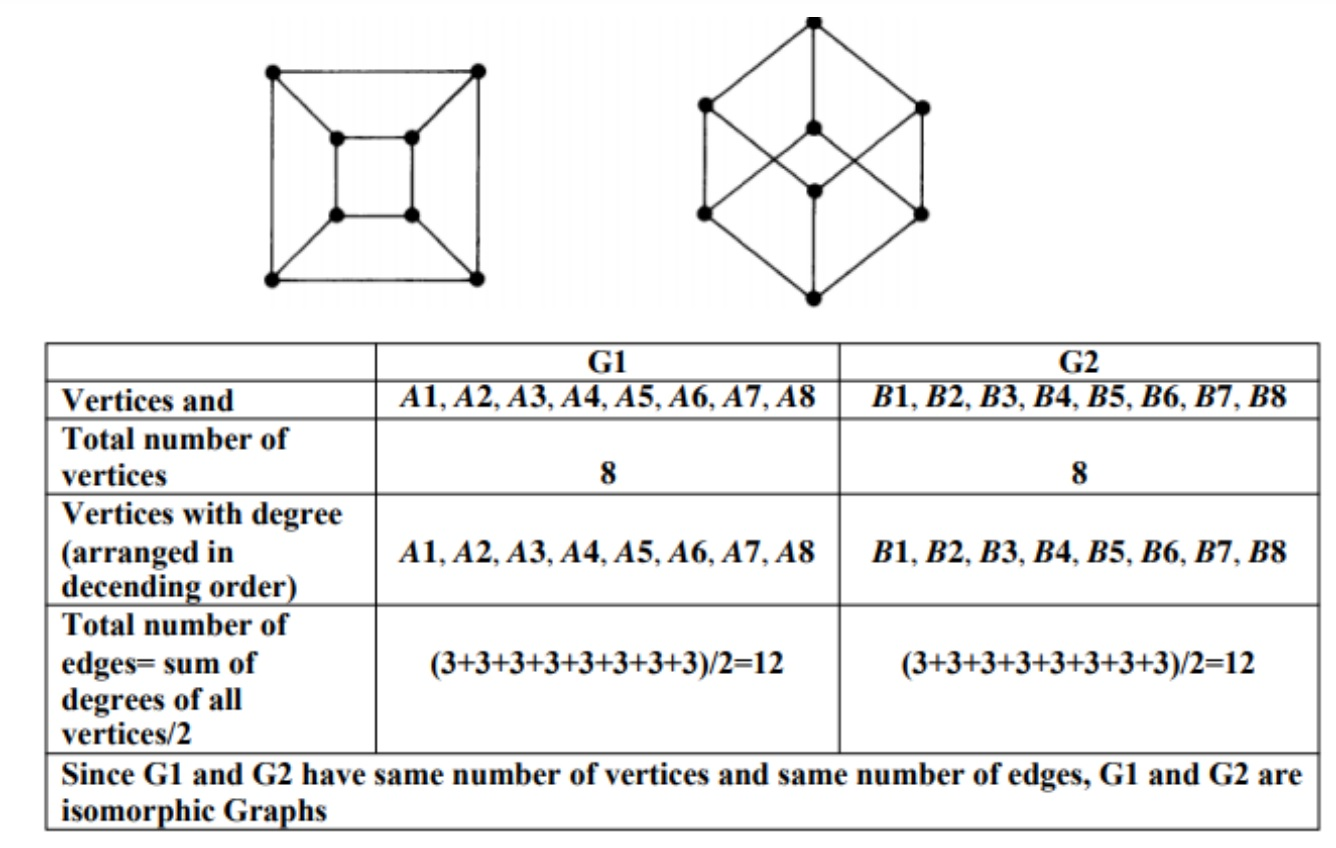
\includegraphics[scale=.4]{img/m40}
	\end{figure}
	
\end{frame}
\begin{frame}{{Isomorphism}}
	
	\begin{figure}
		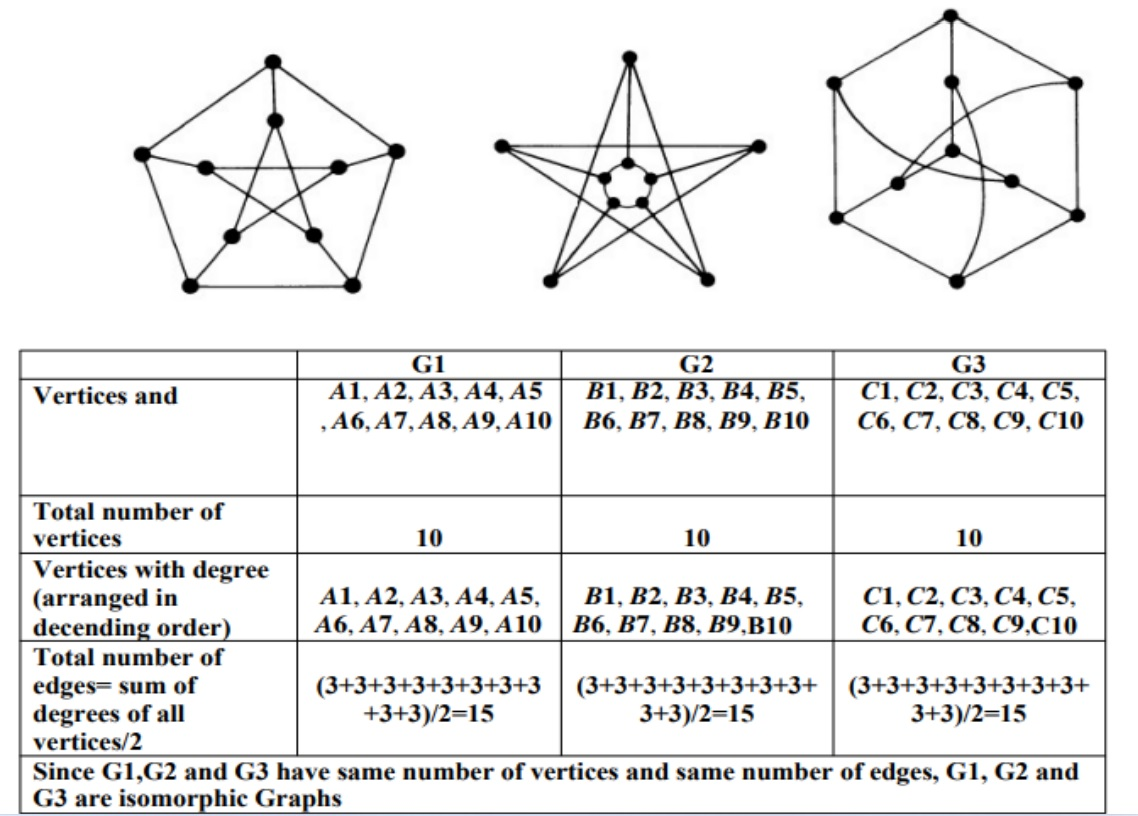
\includegraphics[scale=.4]{img/m41}
	\end{figure}
	
\end{frame}


\begin{frame}{{Isomorphism}}
The following two graphs are not isomorphic, because x is adjacent to two pendant vertex is not preserved.
	\begin{figure}
		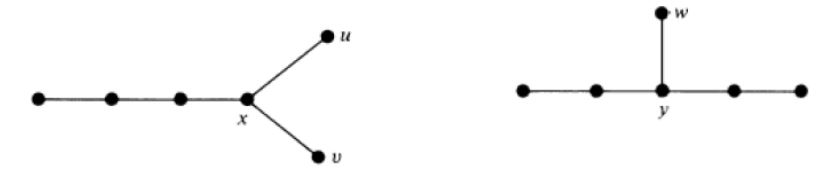
\includegraphics[scale=.5]{img/m22}
	\end{figure}
\end{frame}
\begin{frame}{{Isomorphism}}
	\begin{figure}
		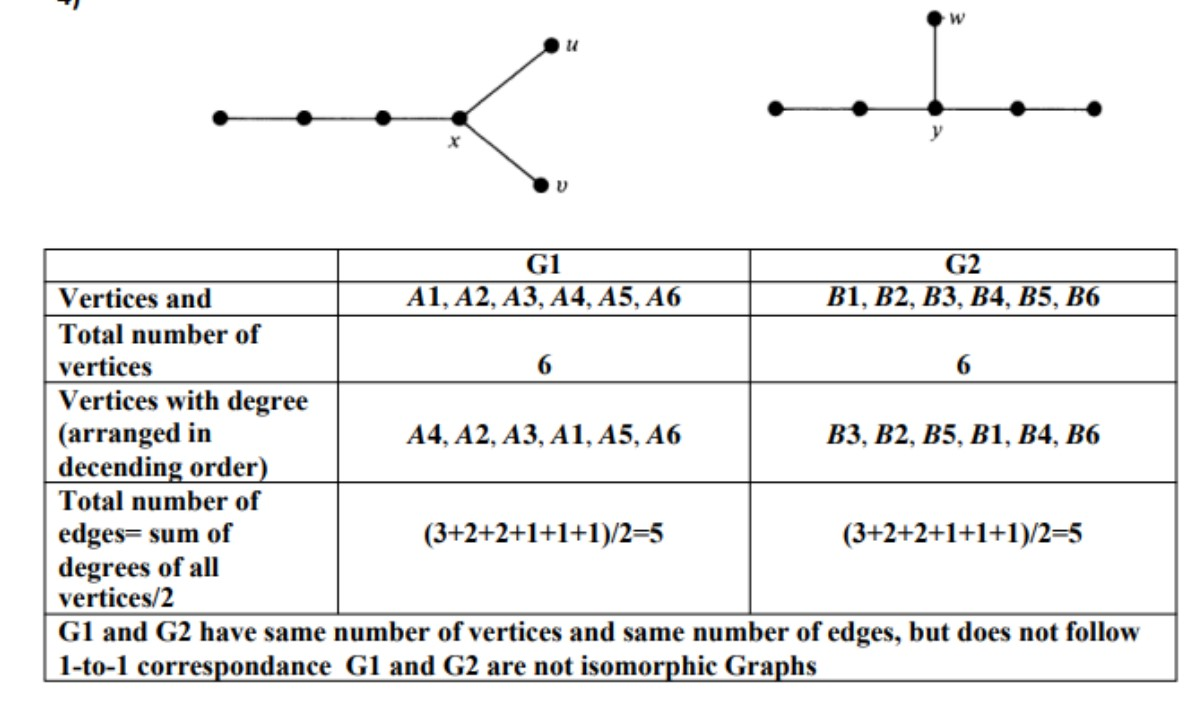
\includegraphics[scale=.45]{img/m42}
	\end{figure}
\end{frame}
\section{Sub graphs}
\begin{frame}{Sub graphs}
	\begin{block}{Sub graphs}
	A graph G' is said to be a subgraph of a graph G, if all the vertices and all the edges 
	of G' are in G, and each edge of G' has the same end vertices in G' as in G.
	\begin{figure}
		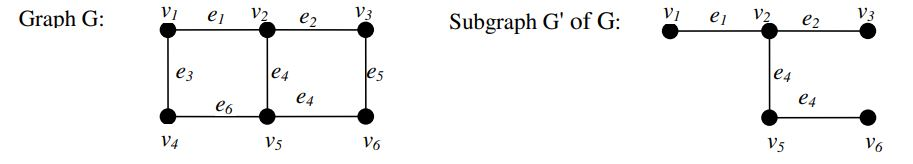
\includegraphics[scale=.5]{img/m23}
	\end{figure}
	\end{block}
\textbf{Properties of sub graph}
\begin{enumerate}
	\item Every graph is its own subgraph. 
	\item A subgraph of a subgraph of G is a subgraph of G. 
	\item A single vertex in a graph C is a subgraph of G. 
	\item A single edge in G, together with its end vertices, is also a subgraph of G. 
\end{enumerate}
\end{frame}
\begin{frame}{Sub graphs}
\textbf{Edge-Disjoint Subgraphs}
\begin{itemize}
	\item Two (or more) subgraphs g1, and g2 of a graph G are said
	to be edge disjoint if g1, and g2 do not have any edges in common.
	\item  The following two graphs are edge-disjoint sub-graphs of the graph G
\end{itemize}
	\begin{figure}
	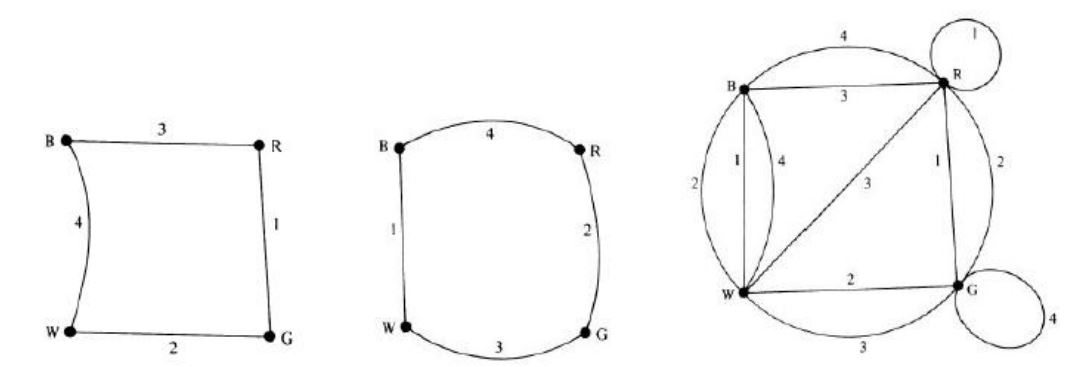
\includegraphics[scale=.4]{img/m24}
\end{figure}
\begin{small}
Note that although edge-disjoint graphs do not have any edge in common, they may have 
vertices in common. \\
\end{small}
\end{frame}
\begin{frame}{Sub graphs}
	\textbf{Vertex disjoint}
	\begin{itemize}
		\item Sub-graphs that do not even have vertices in common are said to be vertex  disjoint.
		\item Obviously they cannot have any edges in common.
		\item p and q are vertex-disjoint subgraphs of G.
	\end{itemize}
	\begin{figure}
	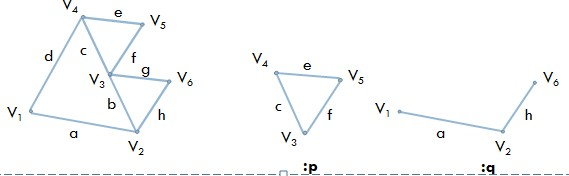
\includegraphics[scale=.6]{img/m28}
\end{figure}
  A subgraph that contains all the vertices of the original graph is called A \textbf{spanning subgraph } .
\end{frame}


\section{Walks, Paths and Circuits}
\begin{frame}{Walks, Paths and Circuits}
	\textbf{Walks/Trail}
	\begin{itemize}
		\item A walk is defined as a finite alternating sequence of vertices and edges, beginning 
		and ending with vertices. 
		\item No edge appears more than once.
		\item It is also called as an edge train 
		or a chain.
	\end{itemize}
\begin{figure}
	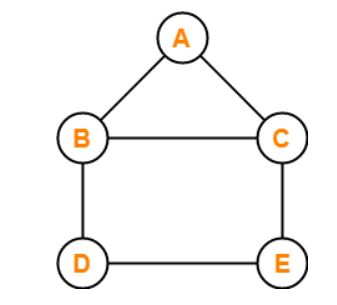
\includegraphics[scale=.4]{img/m25}
\end{figure}
\begin{itemize}
	\item In this graph, few examples of walk are-
	\begin{itemize}
		\item a , b , c , e , d (Length = 4)
		\item d , b , a , c , e , d (Length = 5)
		\item e , c , b , a , c , e , d (Length = 6)
	\end{itemize}
\end{itemize}
\end{frame}
\begin{frame}{Walks, Paths and Circuits}
	\textbf{All about a  Walk/Trail}
	\begin{itemize}
		\item No edge can appear more than once
		\item Vertex may appear more than once
		\item Walk is a sub graph of G
		\item Vertices with which a walk Starts and ends are called terminal vertices of the walk.
	\end{itemize}
\end{frame}

\begin{frame}{Walks, Paths and Circuits}
	\textbf{Walks/Trail}
		\begin{itemize}
			\item \textbf{Closed Walk:} If a walk begins and ends with same vertex, then it is called 
			closed walk
			\item \textbf{Open Walk:} If a walk is not closed is called Open Walk
		\end{itemize}
	\begin{figure}
		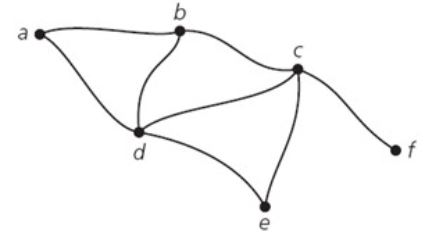
\includegraphics[scale=.5]{img/m26}
	\end{figure}
\begin{itemize}
	\item (b,c),( c,d) and (d,b) provide a b-b (closed walk)
		\item (a,b),(b,c),(c,d), and (d,e) provide a a-e (open walk)
\end{itemize}
\end{frame}



\begin{frame}{Walks, Paths and Circuits}
\textbf{Paths}
\begin{itemize}
	\item An open walk in which no vertex appears more than once is called path.
	\item The 
	number of edges in the path is called length of a path. 
\end{itemize}
\begin{figure}
	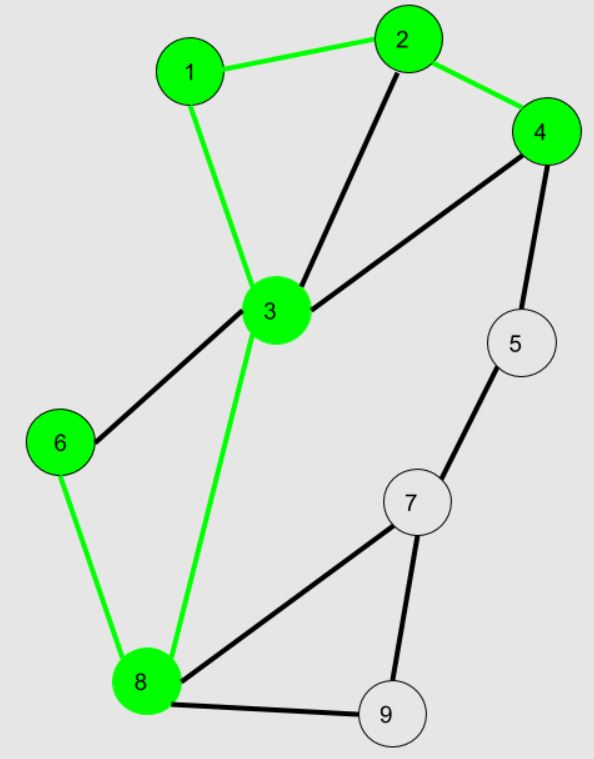
\includegraphics[scale=.2]{img/m27}
\end{figure}
Here $6->8->3->1->2->4$ is a Path\\
Length=5
\end{frame}


\begin{frame}{Walks, Paths and Circuits}
	\textbf{All about a Path }
	\begin{itemize}
		\item No edge can appear more than once
		\item	No vertex can appear more than once
		\item A path of G is a subgraph of G
		\item Starts and ends at different vertices, called the terminal vertices of the path
		\item Terminal vertices are of degree 1
		\item All other vertices are of degree 2
		\item The no. of edges in a path is called its length
		\item An edge itself could be a path
		\item A path is a walk with no vertex repetition
	\end{itemize}
	
\end{frame}


\begin{frame}{Walks, Paths and Circuits}
	\textbf{Circuits/Cycle}
	\begin{itemize}
		\item A closed walk in which no vertex (except initial and final vertex) appears more than 
		once is called a circuit. \item That is, a circuit is a closed, nonintersecting walk. 
		\item Also called as:Cycle, Elementary cycle,
		Circular path, Polygon
	\end{itemize}
	
	\begin{figure}
		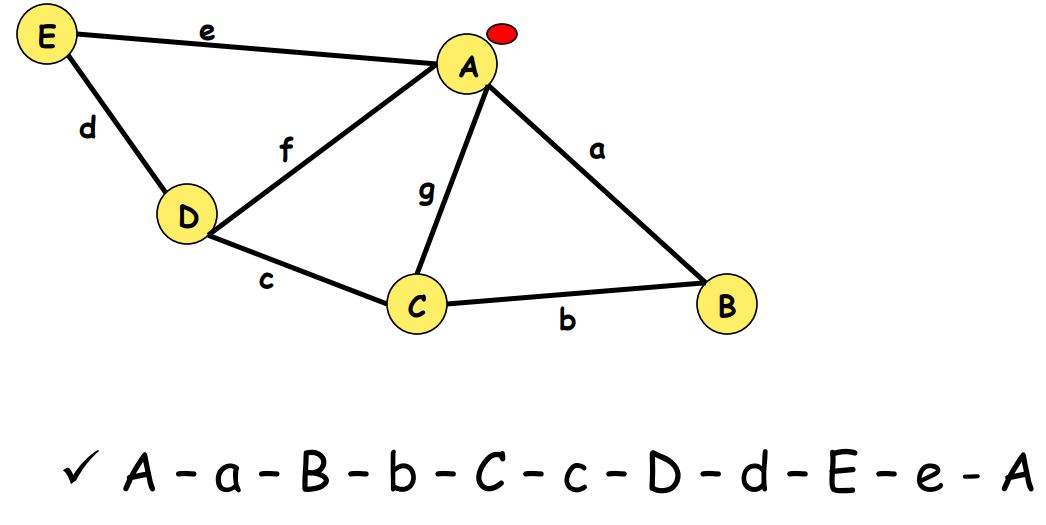
\includegraphics[scale=.3]{img/m31}
	\end{figure}
\end{frame}
\begin{frame}{Walks, Paths and Circuits}
	\begin{figure}
		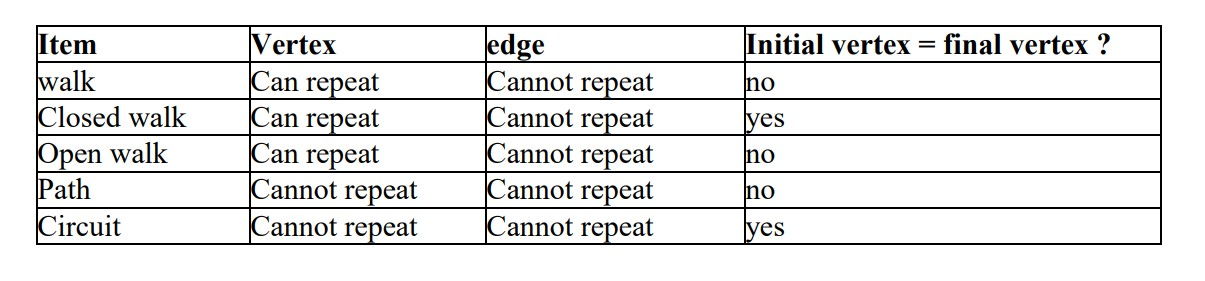
\includegraphics[scale=.5
		]{img/m43}
	\end{figure}
\end{frame}
\begin{frame}{Walks, Paths and Circuits}
	\textbf{Q: In the given graph, trace a}
	\begin{itemize}
		\item Walk
		\item Closed walk         
		\item Path
		\item Circuit 
	\end{itemize}
	
	\begin{figure}
		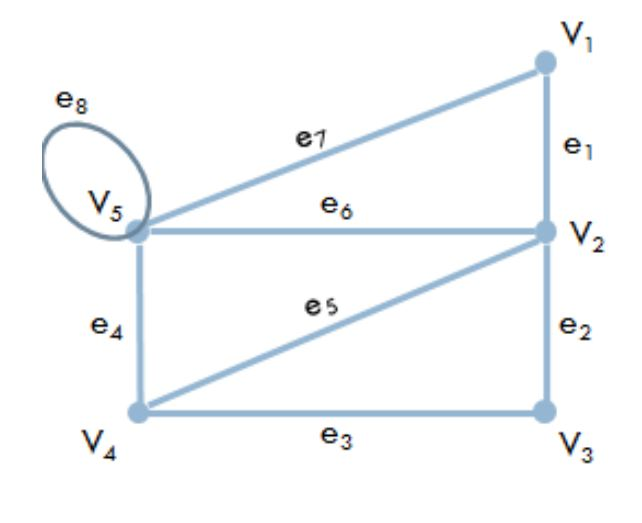
\includegraphics[scale=.4]{img/m32}
	\end{figure}
\end{frame}
\begin{frame}{Walks, Paths and Circuits}
	\textbf{Q: For the given graph H, trace}
	\begin{itemize}
		\item 2 edge disjoint subgraphs
		\item 2 vertex disjoint subgraphs
		\item A walk
		\item A path
		\item A closed walk
		\item A circuit
	\end{itemize}
	
	\begin{figure}
		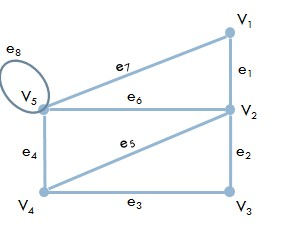
\includegraphics[scale=.6]{img/m33}
	\end{figure}
\end{frame}
\begin{frame}{Walks, Paths and Circuits}
	\textbf{Q:Using the graph classify each sequence as a walk, path or a circuit.}
	\begin{itemize}
		\item E-B-D-E
		\item A-C-D-E-B-A
		\item B-D-E-B-C
		\item A-B-C-D-B-A
	\end{itemize}
	
	\begin{figure}
		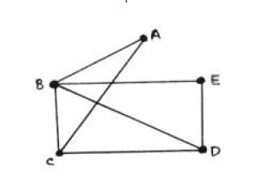
\includegraphics[scale=.6]{img/m34}
	\end{figure}
\end{frame}
\begin{frame}{Walks, Paths and Circuits}
	\begin{figure}
		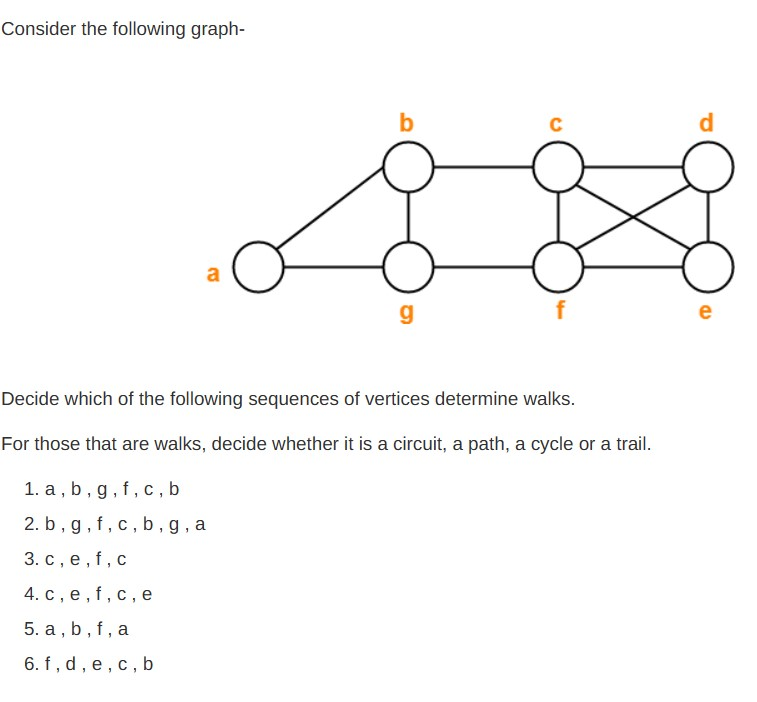
\includegraphics[scale=.55]{img/m44}
	\end{figure}
\end{frame}
\begin{frame}{Walks, Paths and Circuits}
	\begin{figure}
		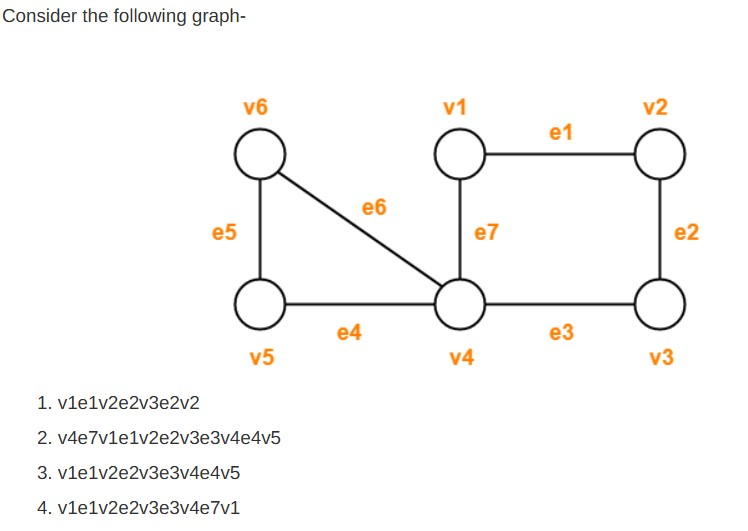
\includegraphics[scale=.6]{img/m46}
	\end{figure}
\end{frame}
\section{Connected Graph,Disconnected Graph \& Components}
\begin{frame}{Connected Graph,Disconnected Graph \& Components}
	\textbf{Connected Graph}
		\begin{itemize}
			\item A graph G is connected if there is at least one path between every pair of vertices in G; else G is disconnected.
			\begin{center}
				Or 
			\end{center}
			\item A graph G is connected if we can reach any vertex from any other vertex
			by travelling along the edges.
		\end{itemize}
		\begin{figure}
		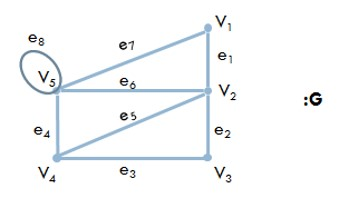
\includegraphics[scale=.6]{img/m35}
	\end{figure}
\end{frame}
\begin{frame}{Connected Graph,Disconnected Graph \& Components}
	\textbf{Disconnected Graph}
	\begin{itemize}
		\item A  disconnected graph consists of two or more connected graphs 
		\item each of these connected subgraphs is called a \textbf{component}.
		\item Hence each component itself is a graph.
	\end{itemize}
	\begin{figure}
		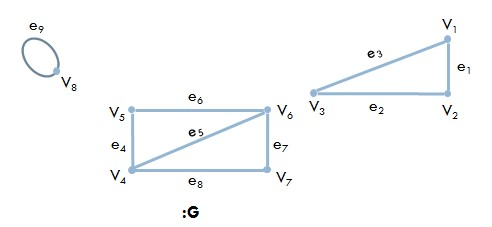
\includegraphics[scale=.6]{img/m36}
	\end{figure}
\end{frame}
\begin{frame}{Connected Graph,Disconnected Graph \& Components}
	\textbf{COMPONENTS }
	\begin{itemize}
		\item A disconnected graph consists of two or more connected graphs. Each of these connected 
		subgraphs is called a component.
	\end{itemize}
	\begin{figure}
		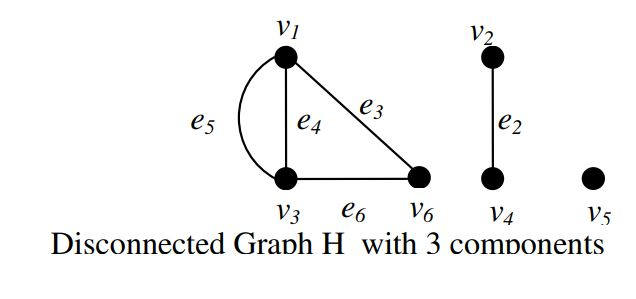
\includegraphics[scale=.6]{img/m37}
	\end{figure}
\end{frame}
\begin{frame}{Connected Graph,Disconnected Graph \& Components}
\begin{block}{THEOREM 1-2}
	A graph G is disconnected if and only if its vertex set V can be partitioned into two 
	nonempty, disjoint subsets $V_1$ and $V_2$ such that there exists no edge in G whose one end 
	vertex is in subset $V_1$ and the other in subset $V_2$.
\end{block}
\textbf{Proof:}\\
$\Rightarrow$
\begin{itemize}
	\item Let  G be a disconnected graph
	\item Consider an arbitary vertex U in G 
	\begin{itemize}
		\item Let $V_1$ be the set of all vertices reachable from U
		\item Since G is disconnected,$V_1$ doesnot contain all the vertices of G.
		\item Let $V_2$ be the set of remaining vertices $V_2=V-V_1$
		\item ie $V_1 \cap V_2=\phi$
		\item No vertex in $V_1$ is joined to any other vertex in $V_2$ by edge
		\item So there is no edge in G whose one end vertex is in $V_1$ and other in $V_2$
	\end{itemize}
\end{itemize}

\end{frame}
\begin{frame}{Connected Graph,Disconnected Graph \& Components}
	\textbf{Proof cont...}\\
	$\Leftarrow$
	\begin{itemize}
		\item Let  G be a graph Whose vertex can be partition in to two nonempty disjoint subsets $V_1$ \& $V_2$
		\begin{itemize}
			\item No edge of G has one end point in $V_1$ and other end point in $V_2$
		\end{itemize}
		\item ie $V_1\cap V_2=\phi$
		
	\item Let u and w be any two vertices in G such that u$\in$$V_1$ and w$\in$$V_2$
	\item There is no path between vertices u \& w, since there is no edge joining
	\item There for the graph is disconnected
	\end{itemize}
\end{frame}
\begin{frame}{Connected Graph,Disconnected Graph \& Components}
\begin{block}{THEOREM 1-3 }
	If a graph (connected or disconnected) has exactly two vertices of odd degree, there 
	must be a path joining these two vertices.
\end{block}
\textbf{Proof:}
\begin{itemize}
	\item Let G be a graph with all even vertices except vertices $v_1$, and $v_2$, which are odd
	\item Since every component of a graph can be considered as a graph itself,  no graph can have an odd number of odd vertices.
	\item Therefore, in graph G, $v_1$ and $v_2$ must 
	belong to the same component
	\item If they lie in the same component there must be a path between them.
\end{itemize}
\end{frame}
\begin{frame}{Connected Graph,Disconnected Graph \& Components}
	\begin{block}{THEOREM 1-4 }
	A simple graph  with n vertices and k 
	components can have at most $$\frac{(n-k)(n-k+1)}{2}$$edges.
	\end{block}
	\textbf{Proof:}
	\begin{itemize}
		\item Let G be a simple graph  with n vertices and k components
		\item let the components be $G_1$,$G_2$,$G_3$,$G_4$.......
		\item Let the number of vertices in $G_i$ be $n_i$
		\item then $n=n_1+n_2+n_3+......+n_k$
	\end{itemize}
\end{frame}
\begin{frame}{Connected Graph,Disconnected Graph \& Components}
	\textbf{Proof cont...}
	\begin{itemize}
		\item The maximum possible number of edges in $G_i$ is
	\end{itemize}
$$\frac{n_i(n_i-1)}{2}$$
\begin{itemize}
	\item Thus maximum number of edges in $G$ is
\end{itemize}
$$\sum_{i=1}^{k}{\frac{n_i(n_i-1)}{2}}=\frac{1}{2}\sum_{i=1}^{k}{n^2}-\frac{1}{2}\sum_{i=1}^{k}{n_i}$$
\end{frame}
\begin{frame}{Connected Graph,Disconnected Graph \& Components}
	\textbf{Proof cont...}
	\begin{itemize}
		\item from algebraic inequality for any set of positive integers $n_1$,$n_2$,$n_3$,$n_4$.......$n_k$
	\end{itemize}
\setcounter{equation}{0}
\begin{equation} 
\sum_{i=1}^{k}{(n_i-1)}= n-k
\end{equation}
squaring both sides(1)
\begin{equation}
	\sum_{i=1}^{k}{(n_i-1)^2}= (n-k)^2
\end{equation}
rewrite(2)
\begin{equation}
	\sum_{i=1}^{k}{n^2}\leq n^2-(k-1)(2n-k)
\end{equation}
\end{frame}

\begin{frame}{Connected Graph,Disconnected Graph \& Components}
	\textbf{Proof cont...}
	\begin{itemize}
		\item  therefor , the maximum number of edges in G is
		\begin{small}
			\begin{eqnarray*}
				\sum_{i=1}^{k}{\frac{n_i(n_i-1)}{2}}&=&\frac{1}{2}\sum_{i=1}^{k}{n^2}-\frac{1}{2}\sum_{i=1}^{k}{n_i}\\
				&=&\frac{1}{2}\sum_{i=1}^{k}{n^2}-\frac{n}{2}\\
				&\leq&\frac{1}{2}[n^2-(k-1)(2n-k)]-\frac{n}{2}\\
				&=&\frac{(n-k)(n-k+1)}{2}\\
			\end{eqnarray*}
		\end{small}
	\end{itemize}
\end{frame}

\begin{frame}{Problems}
	\textbf{At a party of N people, some pair of people are friends with the same number of people at the party.}
	\begin{itemize}
		\item  In a group of N people(vertex), a fellow may have 0, 1, 2, ..., N-1 friends(degrees). Assume to the contrary that all N people have different number of friends. Then for each number in the sequence 0, 1, 2, ..., N-1 there must be a fellow with exactly this number of friends. In particular, there is at least one with N-1 friends. But, if so, all others have this fellow as a friend, implying that there is no one with no friends at all. Therefore, the only possible numbers of friends come from the shortened sequence: 1, 2, 3, ..., N-1. By the Pigeonhole Principle, there are at least two with the same number of friends
	\end{itemize}
\end{frame}
\begin{frame}{Problems}
	\textbf{If 10 people each shake hands with each other, how many handshakes took place? What does this question have to do with graph theory?}
	\begin{itemize}
		\item  This is asking for the number of edges in.  Each vertex (person) has degree (shook hands with) 9 (people). So the sum of the degrees is  90.  However, the degrees count each edge (handshake) twice, so there are 45 edges in the graph. That is how many handshakes took place.
	\end{itemize}
\end{frame}
\end{document}